\documentclass[tikz, border=10pt]{standalone}

\begin{document}
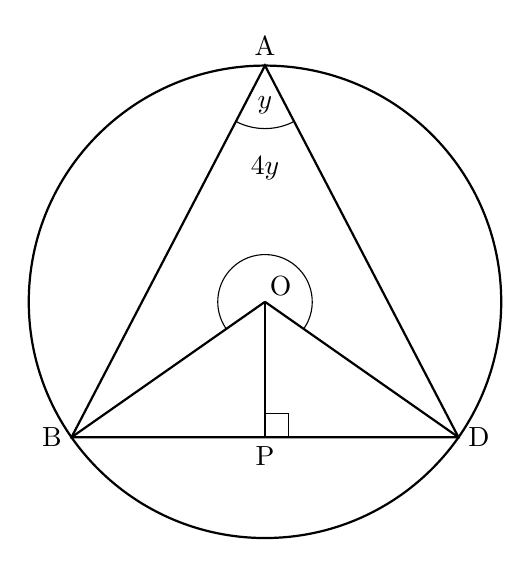
\begin{tikzpicture}[scale=1]

    % 1. Define the center O and radius
    \coordinate (O) at (0,0);
    \def\radius{3}

    % 2. Draw the main circle
    \draw [thick] (O) circle (\radius);

    % 3. Define the main points
    \coordinate (A) at (90:\radius);
    \coordinate (B) at (215:\radius);
    \coordinate (D) at (325:\radius);
    \coordinate (P) at (0,-1.72);

    % 4. Draw Triangle ABD (closed cycle to ensure connection at A)
    \draw [thick] (B) -- (A) -- (D) -- cycle;

    % 5. Draw connecting lines to the center
    \draw [thick] (O) -- (B);
    \draw [thick] (O) -- (D);
    \draw [thick] (O) -- (P);

    % 6. Labels for the points (A, B, D, P)
    \node [above] at (A) {A};
    \node [left] at (B) {B};
    \node [right] at (D) {D};
    \node [below] at (P) {P};

    % 7. Label 'O' - positioned inside the angle O, away from lines
    \node at (0.2, 0.2) {O};

    % 8. Right Angle symbol at P
    \draw (0,-1.42) -- (0.3,-1.42) -- (0.3,-1.72);

    % 9. Angle 'y' at Point A - placed STRICTLY within the arc
    \draw [shift={(A)}] (270-28:0.8) arc (270-28:270+28:0.8);
    \node at (0, 2.5) {$y$};

    % 10. Label '4y' - placed specifically below y and above O
    \node at (0, 1.7) {$4y$};

    % 11. Reflex angle arc at center O
    \draw (325:0.6) arc (325:215+360:0.6);

\end{tikzpicture}
\end{document}
